\documentclass{article}
\usepackage[utf8]{inputenc}
\usepackage{lipsum}
\usepackage[left=2cm, right=2cm, top=3cm, includefoot]{geometry}
\usepackage{comment}
\usepackage {graphicx}%Import images
\usepackage{float}%Set any float position of images for example.
\usepackage{titlepic}
\usepackage{multirow}


\graphicspath{ {\Users\soren\Desktop\Projects 5. semester\Big Data/} }


%Allows for different colors in report
\usepackage{color}
\usepackage[dvipsnames, table, xcdraw]{xcolor}
\usepackage{tabu}
\usepackage{dcolumn}
\newcolumntype{A}{D{.}{.}{2.3}}
\setlength{\parindent}{0pt}


%Setup allows for clickable ToC with different colors
\usepackage{hyperref}
\hypersetup{
    colorlinks,
    citecolor=black,
    filecolor=black,
    linkcolor=black,
    urlcolor=black
}


% Header and Footer Stuff
\usepackage{fancyhdr}
\pagestyle{fancy} %Use fancy page style
\fancyhead[R]{CBS} %Align to the right on the page
\fancyfoot{}
\fancyfoot[R]{\thepage\ } %Align to the right on the page
\renewcommand{\headrulewidth}{0.5pt} %overwrite headers width
\renewcommand{\footrulewidth}{1pt}  %overwrite footers width




\begin{comment}
Renew command overwrites a previous function. Therefore, it is used to overwrite the header and footer width.
fancyfootHDR package, allows us to add cool headers and footers. R aligns to the right  \thepage\ references the actual page number.
\end{comment}




%
\begin{document}





%Start of titlepage
\begin{titlepage}
	\begin{center}
	\line(1,0){300} \\
	[0.25in]
	\color{NavyBlue} \huge{\bfseries A Big Data Research Paper} \\   
	[2mm]	
	\color{black}
	\line(1,0) {200} \\
	[0.1cm]
	\color{black}\textsc{\LARGE On Donald J. Trump's Twitter Activity} \\
	[0.75cm]
	\textsc{\LARGE Copenhagen Business School} \\
	[9.5cm]




\end{center}



\begin{figure}[H]
	\centering

%
 %\raisebox{20mm}[0pt][0pt]{
 %\makebox[\textwidth][c]{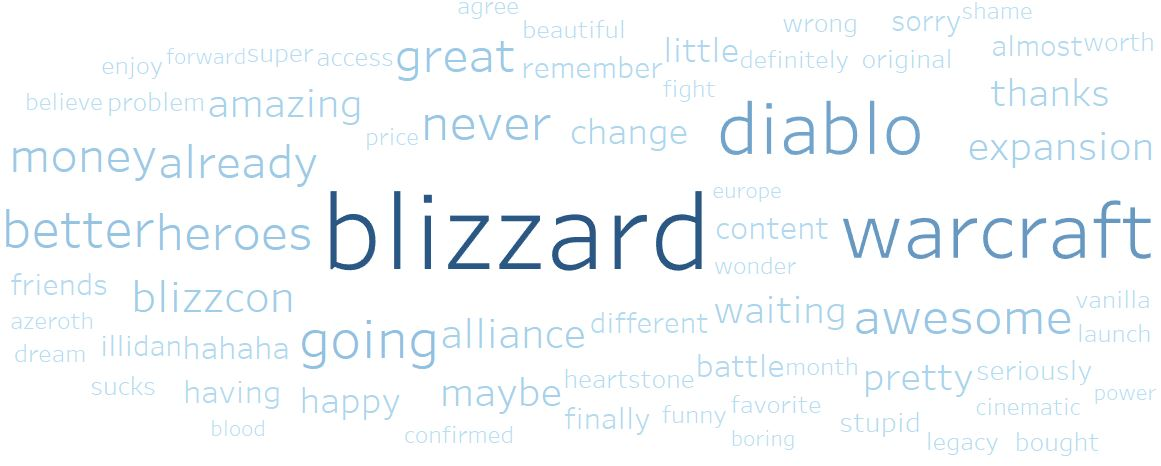
\includegraphics[scale=.55]{BlizzardWord2Cloud.PNG}
 %}}

\vspace*{-12cm} 
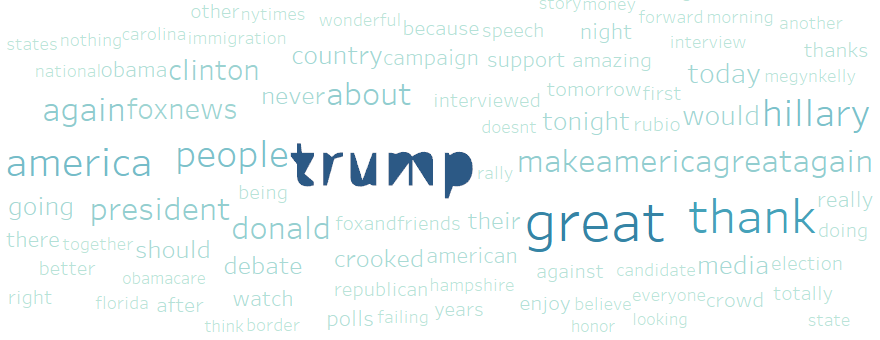
\includegraphics[scale=.75]{TrumpWord.PNG}



\caption{ Trump Wordcloud }
\vspace*{1.25cm} 


\end{figure}


	\begin{flushright}
\vspace*{1.25cm} 

	\textsc{\large Søren Kolbye Jensen \\}
	Bsc. Ha(IT) \\
	\#43124133123 \\
	December 1, 2017
	\end{flushright}





%End of titlepage
\end {titlepage}



%Table of contents & summary
\color{NavyBlue} \tableofcontents \color{black}
\thispagestyle{empty} %Remove the header, by removing all the style
 \cleardoublepage
\setcounter{page}{1}%Reset page counter at introduction page 
\pagenumbering{arabic}
%\addcontentsline{toc}{section}{\numberline{}Summary}


\cleardoublepage%Table of contents end


\section{Summary} %Summary
Summary section


\cleardoublepage %Summary end


%End of table of contents & summary









%Start of report






%Start of introduction_____________________________________________


\color{NavyBlue} \section{Introduction} \label{sec:intro}

\color {black}

Big Data has changed how data is viewed in society, businesses have  invested heavily in infrastructure that can imrpove data collection.
It is now possible, to use Big Data to analyze the behaviour of Social Media channels such as Twitter, Facebook and Instagram. 
However, the vast amount of data available with modern technologies has proven difficult to analyze. According to ??, Big Data can be either
structured or unstructured, where the determining parameters are "Velocity, Verocity and Validity". In order to surmount  this difficulty, new datamining technologies 
has been invented, in order to aid the field of Data Science. \\

These principles are called "Datascience and Datamining". According to (INSERT BOOK), datascience and datamining can be defined as follows: \\

Data science is the act of using fundamental principles, to guide extraction of knowledge from datasets. \\

Datamining on the other hand, deals with extracting knowledge from data using technolgoies, which incorporates the principles of data science.  \\

This research paper, aims to use the fundamental principles of Data science, in conjunction with  datamining technologies.  
To analyze the behvaiour of U.S president Donald J. Trump. and how this behaviour affected his political campaign, as well as how his behaviour affected the American financial markets. The motivation behind this research, is to see how data can reveal a top politians behaviour and thus also discover the actual benefits from Data analysis. 



%Big Data  book ch1






\subsection{Case introduction}
Donald John Trump, born in 1946 in Queens New York, is the CEO of the Trump Organization and is well known as a real-estate broker in the United States.
However, on june 16th, 2015, Trump officially announced his candidacy as the 20th US President". This political campaign was heavily involved with Social Media, as Trump was actively fighting big news channels, such
as CNN, NBC etc. labelling them as "fake news". Thus, Trump figured out a way to distribute highly controversial statements and gain political support by his use of Social Media Channels such as Twitter.\\

I therefore believe that it is extremely relevant to utilize datascience and datamining in order to discover what impact Trump has been able to make on his external environment, by essentially using "distributed data" on the Social Media Network: Twitter. 



%http://secfilings.nasdaq.com/edgar_conv_html%2f2017%2f02%2f28%2f0001047469-17-001072.html#FIS_BUSINESS

\cleardoublepage



%End of introduction________________________________

%https://www.aol.com/2016-election/timeline/
%https://www.dropbox.com/sh/kd87npmrvcwiyge/AADRTmSB6lDt5ChunVY_Xy0Ea/ExampleProjects?dl=0&preview=ExampleProject%2301-VisualAnalytics-NYC_TaxiRides-GreenCabs_vs_Uber.pdf

\section{Problem Formulation and Reserach questions} \label{sec:ch1}
The goal of this research paper is to analyze  trumps behaviour on Twitter and how he used Twitter to combat "fake news". A visual analysis on his behaviour between DATE and DATE will be conducted to reveal the patterns in his behaviour in this timeframe. This leads to the reserach question: 

\par\vspace{10pt}

What was trump's behaviour on social media, prior to his announcement of his presidency. And how did it change, during and after his political campaign.\\

In addition to this, due to Trump's political position, it would be interesting to investigate the impact that his tweets has on the stockprice of companies, during his campaign he has posted both good and bad things about nurmerous companies. It is therefore relevant to investigate, if his Tweets have an impact and if that impact is short-term or long-term. This leads to the research question:\\

How does Trump's behaviour affect the stock prices of companies ? \\

Finally, it is relevant to evaluate and discuss what the above actually means to the context of Data Science, both from an ethical point of view, but also from a practical point of view. This leads to the final research question: \\

What does Donald Trump's behaviour mean from a datascience standpoint and how do we avoid ethical implications?
 



\section{Theoretical Framework}
In this section I will discuss my theoritcal framework which I used in order to investigate the research questions using data science. Some aspects of this chapter, may "transition" into the realm of methodology, but are none the less relevant to mention in both contexts.


\subsection{Supervised datamining}
Supervised and unsupervised datamining comes from machine learning, in a supervised method the data scientist will "supervise" the data and provide target information. In this research paper I have chosen to use supervised datamining, because I had a specific target.  There are two "main" subclasses when it comes to using supervised data mining. One is classification and the other is regression - these two differ in terms of what the target is. In this research paper, the target is stock prices and thus it can be defined as a numeric target. The other main subclass of supervised datamining is classification which deals with binary targets, however this has not been used in the reserach paper.

I will use supervised datamining methods, because my target is specified and the data on said target exists. Furthermore, the historical data of the stock value of the examined companies are complete.



\subsection{Linear regression and fitting}
In this research paper, models containing linear regressions will be used, in order to discover the relationship among variables in the data model.  This will help create a simple predictive model of the datasets showcasing Trump's short-term impact on certain companies, when he tweets about them, in a negative or positive way. In these regressional models, the x-variable will be the date the tweet was posted and the y-variable will be the closing price of a given stock. Thus, resulting Lienar  Functions with the format : y=mx+b, where m is the slope and b is where y intercepts. This will be done by attempting to fit a linear relationship between the dependent (Y) and independent (X) variables. \\

There are other regressional models that can be used with supervised datamining. The use of statistical methods can be used, in order to discover which model has the best fit to your dataset. Such as  R-squared values, but in this research paper only linear regression will be used due to time constraints and my own lack of practical knowledge to complete a more statistically advanced model. However, the R-squared values will be discussed in the report, in order to examine the fit. \\

In order to illustrate the importance of the R-squared value, the term overfitting and underfitting  datasets has to be defined. \\

Overfitting is when a datamining procedure is completely tailored to the training data, in a worst case it is because a model is "memorized". This has a cost in terms of achieving a model that can generalize in terms of unseen data points and it may result in poor model performance and harmful consequences when determining correlations in a dataset. 

 According to the authors of the books, overfitting is unavoidable to some extend. Therefore, there is not a specific data mining precdure that is "best" in terms of overfitting, nor does the authors argue that the answer is to produce a more simply model in order to produce less overfitting. There is a trade-off when making more complex models and overfitting, it depends on the situation and such a decision must be considered throughly by the data scientist, if a model is too simple it may not convey the actual complexities and thus will be less accurate than an advanced model with more overfitting.
In terms of this report, I have decided that a simple linear regression is enough in order to get the bigger picture of Trump's short term impact on a companies stock, although I cannot deny that a more complex data model with more overfitting may have yielded better results. \\

* Underfitting
The opposite of overfitting is if we have a model that is underfitting. This means that the model that was produced is not good enough to represent the fitted data.  In terms of the R-squared value, the lower it is the more the model will be underfitting and the less useful the model will be in terms of representing the data.


https://www.pugetsystems.com/labs/hpc/Machine-Learning-and-Data-Science-Linear-Regression-Part-6-978/



%https://cloudtweaks.com/2014/09/use-supervised-unsupervised-data-mining/

%Methodology start

\section{Methodology}
To answer the research questions two different types of analysis is presented\\


Furthermore,  the CRISP framework has been used in a modified fashion, in order to better illustrate the context of this research paper.\\

\begin{figure}[H] %We begin our figure and want it to stay H(ere)
	\centering %We want to center the figure
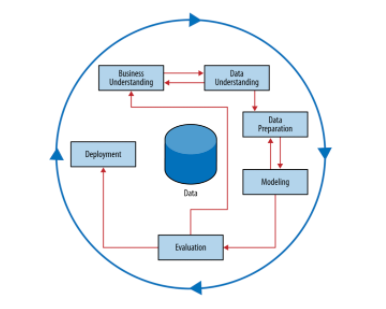
\includegraphics [scale= .95]  {CRISP.PNG}    %Include our ijmage with a height and location of img.
	\caption[Optional caption] {real, local caption for refrence}
	\label{fig:wordcloudBliz}

\end{figure}


The model serves to illustrate how the data was processed throughout the proejct in order to yield a final result/answer to the research questions. The model is iterative and serves to explore the Twitter data, so a better
understanding of the data can be reached. This process has been conciously iterated throughout the project.

"Business understanding" is in this context the overall problem formulation and research questions that we wish answered.\\
For every iteration a deeper understanding of the data is achieved, which affects the understanding of the overall research framework.\\

Data Understanding is how we collect the data from raw material and build a solution, it is therefore essential to critique your data and see what strengths and weaknesses that the data has. It can also be relevant to estimate the cost of the data, especially in a business context. However, for the purposes of this specific research paper, the economical aspect of data collection such as Cost/benefit won't be explored. Due to the iterative nature of the CRISP framework, different solutions may change the direction of the analysis. The essential part to take away from this, is that we use data understanding in order to get a deeper understanding of our data and thus discover what the structure of the data is and how it can be used to "solve" what in this research question is our business problem/research questions.


"Data preparation" is where we merge, cleanse and integrate multiple data sources. In this research paper, Alteryx has been used as shown in Table 1 later in the report.
"Modelling has used Tableau, which is a visual analytics tool. This makes it easier to explore and understand the patterns presented in the data. It has been a very closely fit process together with data understanding, in order to achieve the best results of "good" data (In this case, usable data that can answer our research questions)  and how to prepare it (So that frontend programs can be used in order to visualize  findings) \\

Modelling is what we end up with, it is here our overall "model" is made which captures patterns and regularities within the data. It is the stage where most data mining tehcniques are applied in order to create a model that is usable.

"Evaluation" Here we evaluate, whether the data model that has been built answers the overall research questions. After the model has been evaluated and validated, the model will go through "deployment", which in this sense will be the final conclusion to
the research questions.\\


\subsection {My overall process of handling data}

I have developed the following model, to ilustrate how I have used Alteryx and Tableau in order to build a model. I have also attempted to illustrate how I used the CRISP model here, by determining if a given model is satisfactory. If not, I go back to the drawing board and reconsider what data I have and how I can prepare it in Alteryx, so that I can build a new model through the next iteration.



\begin{figure}[H] %We begin our figure and want it to stay H(ere)
	\centering %We want to center the figure
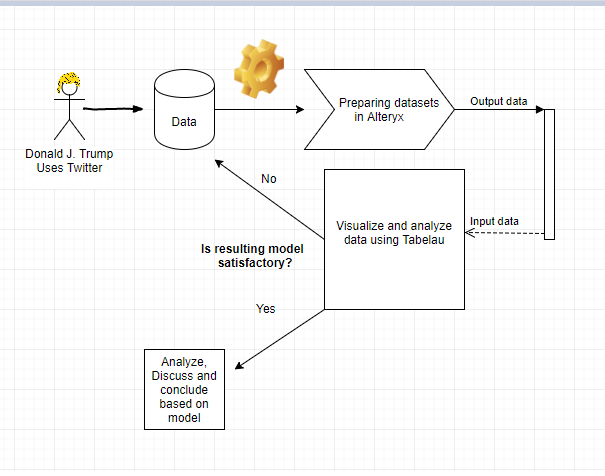
\includegraphics [scale= .85]  {SygModel.PNG}    %Include our ijmage with a height and location of img.
	\caption[Optional caption] {real, local caption for refrence}
	\label{fig:wordcloudBliz}

\end{figure}


Throughout this project, I have attempted numerous models, most of which were discarded. Such as determining which fake news trump tweets most about, because I did not feel it answered the overall research question further.










%Table
%https://www.alteryx.com/analytics/data-mining-software

%Data Analytics tool that provide data mining solutions
% by helping with data cleansing and integration 
%of multiple sources.
%This tool helps with visual data representations in a 
%dynamic environment, where several datasets can be
%joined in order to create a comprehensive data solution.
 To summarize, Table 1 shows the purpose and use of each datamining tool used in this research paper: 


\begin{table}[H]
\centering
\caption{My caption}
\label{my-label}
\begin{tabular}{|l|l|l|l|l|}
\hline
\rowcolor[HTML]{656565} 
{\color[HTML]{000000} \textbf{Tool:}} & {\color[HTML]{000000} \textbf{Purpose:}} & \multicolumn{3}{l|}{\cellcolor[HTML]{656565}{\color[HTML]{000000} \textbf{Use:}}} \\ \hline
\rowcolor[HTML]{BBDAFF} 
\cellcolor[HTML]{BBDAFF}{\color[HTML]{000000} } & \cellcolor[HTML]{BBDAFF}{\color[HTML]{000000} } & \multicolumn{3}{l|}{\cellcolor[HTML]{BBDAFF}{\color[HTML]{000000} }} \\
\rowcolor[HTML]{BBDAFF} 
\cellcolor[HTML]{BBDAFF}{\color[HTML]{000000} } & \cellcolor[HTML]{BBDAFF}{\color[HTML]{000000} } & \multicolumn{3}{l|}{\cellcolor[HTML]{BBDAFF}{\color[HTML]{000000} }} \\
\rowcolor[HTML]{BBDAFF} 
\multirow{-3}{*}{\cellcolor[HTML]{BBDAFF}{\color[HTML]{000000} \textbf{Alteryx}}} & \multirow{-3}{*}{\cellcolor[HTML]{BBDAFF}{\color[HTML]{000000} \begin{tabular}[c]{@{}l@{}}Data Analytics tool that \\ provide data mining solutions\\  by helping with data \\ cleansing and integration \\ of multiple sources.\end{tabular}}} & \multicolumn{3}{l|}{\multirow{-3}{*}{\cellcolor[HTML]{BBDAFF}{\color[HTML]{000000} \begin{tabular}[c]{@{}l@{}}Lorem ipsumLorem ipsumLorem \\ ipsumLorem ipsum\\ Lorem ipsumLorem ipsumLorem ipsum\end{tabular}}}} \\ \hline
\rowcolor[HTML]{BBDAFF} 
\cellcolor[HTML]{BBDAFF}{\color[HTML]{000000} } & \cellcolor[HTML]{BBDAFF}{\color[HTML]{000000} } & \multicolumn{3}{l|}{\cellcolor[HTML]{BBDAFF}{\color[HTML]{000000} }} \\
\rowcolor[HTML]{BBDAFF} 
\cellcolor[HTML]{BBDAFF}{\color[HTML]{000000} } & \cellcolor[HTML]{BBDAFF}{\color[HTML]{000000} } & \multicolumn{3}{l|}{\cellcolor[HTML]{BBDAFF}{\color[HTML]{000000} }} \\
\rowcolor[HTML]{BBDAFF} 
\multirow{-3}{*}{\cellcolor[HTML]{BBDAFF}{\color[HTML]{000000} \textbf{Tableau}}} & \multirow{-3}{*}{\cellcolor[HTML]{BBDAFF}{\color[HTML]{000000} \begin{tabular}[c]{@{}l@{}}This tool helps with visual\\ data representation.\end{tabular}}} & \multicolumn{3}{l|}{\multirow{-3}{*}{\cellcolor[HTML]{BBDAFF}{\color[HTML]{000000} \begin{tabular}[c]{@{}l@{}}Lorem ipsumLorem ipsumLore\\ m iLorem ipsumpsumdasdLo\\ remLorem ipsum ipsum\end{tabular}}}} \\ \hline
\end{tabular}
\end{table}


\subsection{Data Acquisition and Dataset Description}
The datasets in this research paper has been collected from Trump's Twitter page, ranging from 2009 to 2017.

The first datasets consists of Twitter data on Trump's primary twitter channel.  This dataset will mainly be used to analyze Trump and his Campaign team's behaivour. 

The second dataset consists of Historical data on the American and Mexican currency between Trump's announcement to  14/07/2017

The third dataset is collected through Sentione and will be used to analyze the sentiment towards Trump's campaign. Ranging from before his inauguration, until 02/11/2017. 

\cleardoublepage


\section{Results}
In this section of the research paper, I will go through the results of my datamining and discuss it in relation to the research question, and thus explain which insights I came across during my datamining, in order to create a meaningful discussion regarding Donald J. Trump's behaviour and impact on the stock prices of companies. The result section will be built around the CRISP framework, in order to better illustrate the process of my datamining.

\subsection{Business understanding and Data Understanding}
The understanding of both the overall research questions / Problem statement and the data was a very iterative process and thus is hard to document in a research paper, therefore my understanding will mostly be reflected in the following sections, where my ideas and reflections will be discussed.  And hopefully create a reflection of how I arrived at the understand of both my research questions and the data.

\subsection{Data Preperation}
In order to prepare the Datasets from Twitter and Sentione, I used a datamining tool called "Alteryx", which deals with the backend part of the data analysis. This tool was used to filter my data and join the relevant tables with each other, in order to make a comprehensive analysis. Data that was filtered out was things such as "Twitter ID" and "URL", as these were not needed for the direction I was going for. 

Furthermore, numerous WordClouds were produced with the Alteryx tool, by extracting the text-value of Trump's tweets, 



\section{To be added later}

As shown in Figure X, Trump makes a tweet about an aircraft company, who supplied to the US. Government?, the result of his negative tweet, the company stock had a short-term impact and dropped on the next close-price. Starting out at a close-price of xxxx at xxxx and ended up with a close-price of xxxx after Trump's Tweet the xx/xx/xx \\

To dig deeper and analyze Trump's behavior even further, we can use Text-mining in order to determine the most frequently words that he used. Here we can see that before he announced his candidacy, he was already very invested in politics and tweeted mostly about Obama and making America great again. Looking at the text-mining during his presidency, the most frequently words that pop up are mostly of Hillary along with "nicknames" such as "crooked" that Trump used during his campaign in order to ?denounce his political opponents.  \\


Furthermore, by the use of text-mining and using an algorithm, that sorts comments into differerent classifications "positive", "negative", "neutral". It is possible to determine, whether the reaction of Trump's presidency was overall positive or negative. \\

The results show that Trump's inital support at the announcement of his presidency was overall positive, with very few negative comments.  The negative comments grew exponentially, as Trump got closed to winning his presidency, peaking around the time of his inagruation at xx/xx/xxxx




%End of report__________________________________



\end{document}






%\begin{figure}[H] %We begin our figure and want it to stay H(ere)
%	\centering %We want to center the figure


 %\raisebox{10mm}[0pt][0pt]{
%\fbox{ \makebox[\textwidth][c]{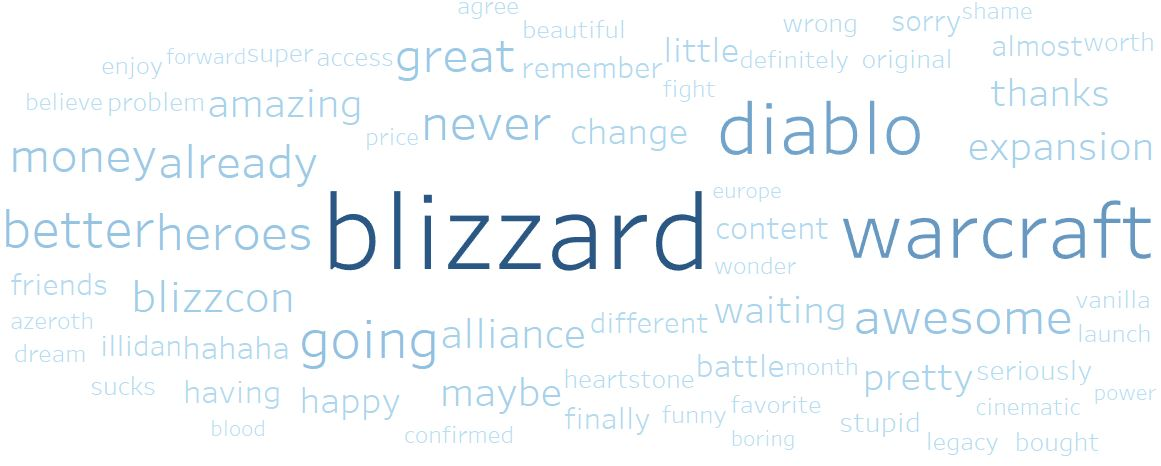
\includegraphics[scale=.55]{BlizzardWord2Cloud.PNG}}
% }}
%\vspace*{-40mm} %Close in the caption to the image

%\protect\caption[position=bottom]{Title of Figure\label{fig:F1}}


%\vspace{3cm}
%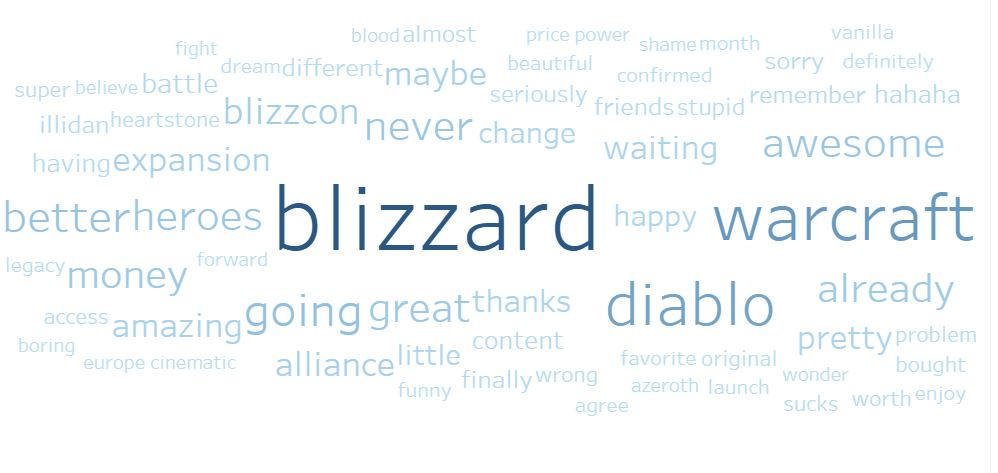
\includegraphics [width = 7in]  {BlizzardWordCloud.PNG}     %Include our ijmage with a height and location of img.
	
%	\label{fig:wordcloudBliz}

%\end{figure}



